\section{Mobile Application Security}

\subsection{iOS}
Basierend auf OSX hat Apple das iOS lanciert. Dabei wurde Objective-C, Swift, und C verwendet. iOS verfügt über Sandbox Mechanismen, ein Data Protection API, Code Signing und den Appstore mit manueller Freischaltung.

\begin{figure}[H]
	\centering
	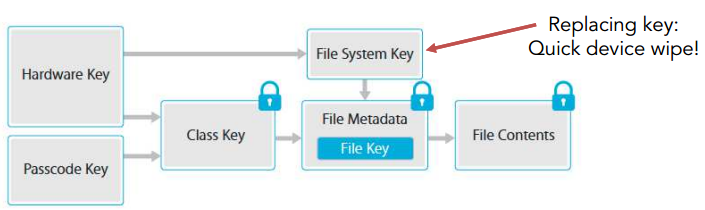
\includegraphics[width=0.6\textwidth]{./img/mobileappsecurity_iOS-DataProtectionAPI}
	\caption{iOS Data Protection API}
\end{figure}

Bei iOS ist das \textbf{Permission Model} so eingerichtet, dass bei jeder Verwendung nach Erlaubnis gefragt wird und individuell erlaubt oder abgelehnt werden kann.

\subsection{Android}
Auf Linux basierend in Java und C entstand Andoid, welches von verschiedene Hardware-Anbietern übernommen wurde. Somit hat es auch noch viele alte Versionen auf dem Markt.

Android unterstützt SD Karten, Sandboxing via JVMs, Code Signing, und mehrere verschiedene Appstores.

Die \textbf{App Permissions} sind bei Android im Manifest hinterlegt und können ab Android 6 individuell angenommen oder abgelehnt werden.

\subsection{Windows Phone}
Windows Phone von Microsoft unterstützt ebenfalls strict sandboxing, Address Space Layout Randomization (ASLR, zufällige Ladeposition von Programmen in Speicher als Schutz gegen Overflow), Bit Locker Verschlüsselung, Data Protection API (ähnlich wie bei iOS), aber auch Gefahren wie automatisches Wi-Fi credential sharing über Facebook, Outlook oder Skype.

\subsection{Xamarin}
Xamarin ermöglicht die Entwicklung von platformübergreifenden, nativen Apps. Dabei wird das .NET Framework verwendet und in C\# programmiert, welches zu IL-Code (Microsoft Intermediate Language) kompiliert wird.

Die native APIs werden zwar zu den .NET namespaces gemapped, jedoch müssen platformabhängige Security Features immer noch für jede Platform geschrieben werden.

\subsection{Cordova (Phonegap)}
Cordova wird verwendet um Mobile Apps mit HTML, JS und CSS zu entwickeln. Es bringt somit native Funktionalität, basiert aber auf Web View Komponente. Somit fallen jedoch auch alle bekannten Schwachstellen an.

\section{OWASP Mobile Top 10}
\todo[inline]{OWASP Mobile Top Ten}
\begin{figure}[H]
	\centering
	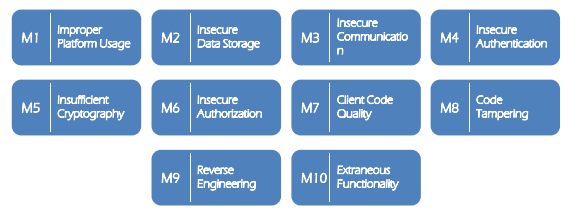
\includegraphics[width=0.6\textwidth]{./img/OWASP_MobileTop10}
	\caption{OWASP Mobile Top 10, 2016}
\end{figure}

\subsection{M1: Improper Platform Usage}
Missbrauch eines Platform Features oder fehlende Sicherheitsmassnahmen, und das somitige Verletzten von Guidelines. \\

\textbf{Beispiel}: Zu viele Permissions, unverschlüsseltes Ablegen von Credentials in Property-File anstelle der KeyChain (iOS). \\

\textbf{Lösung}: Konsultieren von Guidelines beim Entwickeln.

\subsection{M2: Insecure Data Storage}
Durch Ablegen von Daten in unsicherem Speicher oder unvorhergesehenem Datenleak (siehe Unterkapitel) besteht erhöhte Gefahr wenn das Gerät gestohlen wird/verloren geht oder mit Malware infiziert ist nach jailbreak/rooting.

\subsubsection{System Screenshots}
Beim Wechseln zwischen Apps wird ein Screenshot sichtbar um zu sehen was die App zuletzt dargestellt hat. \\

\textbf{Beispiel}: E-Banking Kontoinformationen können eingesehen werden über den Screenshot des Apps. \\

\textbf{Lösung}: Screenshots vom System unterbinden oder sensitiven Daten überdecken.
\begin{lstlisting}[language=C, caption=Lösung für iOS]
(void) applicationDidEnterBackground:(UIApplication *)application{
	// mask the sensitive data or add an additional layer on top			
}
\end{lstlisting}
\begin{lstlisting}[language=Java, caption=Lösung für Android]
window.addFlags(LayoutParams.FLAG_SECURE, LayoutParams.FLAG_SECURE);
\end{lstlisting}

\subsubsection{Keyboard}
Viele Keyboards verfügen über Autocomplete. Das iOS zum Beispiel speichert bis zu 500 Wörter.\\

\textbf{Beispiel}: Passwort Feld unterstütz Autocomplete; Das Passwort wird somit auch an anderen Stellen vorgeschlagen wenn mit dem selben Buchstaben begonnen wird. \\

\textbf{Lösung}: Autocomplete bei sensitiven Daten deaktivieren.
\begin{lstlisting}[language=C, caption=Lösung für iOS]
theTextField.secureEntry = YES;
theTextField.autocorrectionType = UITextAutocorrectionTypeNo;
\end{lstlisting}
\begin{lstlisting}[language=Java, caption=Lösung für Android]
android:inputType="textNoSuggestions";
\end{lstlisting}

\subsubsection{Clipboard}
Standardmässig wird ein globales Clipboard für Copy \& Paste verwendet, und jedes App kann darauf zugreifen. \\
\textbf{Beispiel}: Sensitive Daten befinden sich noch im Clipboard aus der E-Banking App.

\textbf{Lösung}: Clipboard leeren oder ein dediziertes Clipboard verwenden.
\begin{lstlisting}[language=C, caption=Lösung für iOS]
UIPasteBoard *uniqueBoard=[UIPasteboard pasteboardWithUniqueName];
\end{lstlisting}

\subsubsection{Logs}
Crash und App logs können sensitive Daten enthalten. Im Apple System Log (ASL) bei iOS werden sogar alle Logs gecached bis zum nächsten Reboot und auch nicht sandboxed. Bei Android müssen Debug Logs bei der finalen App deaktivieren werden. \\

\textbf{Beispiel}: Bei gescheitertem Loginversuch speichert das Log Benutzername und Passwort im Log. \\

\textbf{Lösung}: Dedizierter Logger für Debug Build der App.

\subsubsection{Web Data}
Eine WebView speichert jegliche Daten wie ein konventioneller Web Browser. Dies umfasst ein Web Cache, lokaler Speicher, Cookies, Passwörter die direkt oder in eine Sqlite Datenbank gespeichert werden. \\

\textbf{Beispiel}: Ablegen von unverschlüsselten Passwörtern und Benutzernamen in Sqlite Datenbank.\\

\textbf{Lösung}: Korrekte Systemspeicher verwenden.

\subsubsection{Inter-Process Communication}
Apps können URL Handlers registrieren, der Empfänger und die überlieferten Informationen werden aber nicht überprüft. Zudem entsteht ein Problem wenn mehrere Apps für ein Handler bestehen. Bei Android kann dann die aufzurufende Applikation gewählt werden, bei iOS wird die zuletzt installierte App automatisch ausgewählt.\\

\textbf{Beispiel}: Sensitive Daten werden bei Aufruf über einen Handler abgefangen.
\begin{lstlisting}[language=XML, caption=Aufruf von Skype]
skype://090012312312?call
\end{lstlisting}

\textbf{Lösung}: Bei Android direkter Aufruf eines Intent aus der anderen App.

\subsection{M3: Insecure Communication}
Das Verwenden von inkorrekten oder alten SSL Versionen, schwache Protokollaushandlung oder einfach Plain Text Kommunikation.

Ab iOS 9 wurde mit \textbf{App Transport Security} durch mimimum Anforderungen eingeführt (TLS 1.2 mit PFS, Zertifikat und SHA-256 Signatur, 2048-bit RSA oder 256-EC Key). Apps unterstehen diesen Vorbestimmungen oder müssen explizite Ausnahmen definieren.

\subsubsection{Certificate Pinning}
Standardmässig wird bestimmten Certificate Authorities (CA) vertraut. Deren Root Zertifikate sind auf jedem Gerät vorinstalliert.\\

\textbf{Beispiel}: Die CA wurde gehacked oder ein Attackierer hat dem Gerät eine falsche CA hinzugefügt. \\

\textbf{Lösung}: Certificate Pinning, eingeführt durch Google Chrome. Speichert das Zertifikat oder dessen Public Key in der App und überprüft dieses.

\subsection{M4: Insecure Authentication}

\subsection{M5: Insufficient Cryptography}

\subsection{M6: Insecure Authorization}

\subsection{M7: Client Code Quality}

\subsection{M8: Code Tampering}

\subsection{M9: Reverse Engineering}

\subsection{M10: Extraneous Functionality}
\subsection{Checkliste}

